%%% DOCUMENT CONFIGURATION %%%

\documentclass[
	letterpaper, % Paper size, use either a4paper or letterpaper
	10pt, % Default font size, can also use 11pt or 12pt, although this is not recommended
	unnumberedsections, % Comment to enable section numbering
	twoside, % Two side traditional mode where headers and footers change between odd and even pages, comment this option to make them fixed
]{LTJournalArticle}

\addbibresource{sample.bib} % BibLaTeX bibliography file

\setcounter{page}{1} % The page number of the first page, set this to a higher number if the article is to be part of an issue or larger work

\usepackage{amsmath}

%%% TITLE SECTION %%%

\title{Leveraging Neural Networks for Efficient Obstacle\\Avoidance and Racing an Autonomous Car}
% Article title, use manual lines breaks (\\) to beautify the layout

\author{Yanxiang Zhang, Chaarvi Goel, Siddharth H. Nair, Francesco Borrelli
\thanks{\;Y. Zhang and C. Goel are with the Department of Electrical Engineering and Computer Sciences, S. H. Nair is with the Department of Mechanical Engineering, University of California, Berkeley, Berkeley, CA 94701, USA \texttt{\{joshzhang, chaarvigoel, siddharth\_nair, fborrelli\}@berkeley.edu}}}

\date{}    % This prevents a bug idk
\begin{document}
\maketitle % Output the title section

%%% ARTICLE CONTENTS %%%

\textbf{\small\textit{Abstract}---In this paper we present a novel neural network model capable of predicting a large number of output dimensions from minimal input data. This research addresses the challenges in autonomous car technology, particularly in high-speed environments with limited visibility. The model, developed using PyTorch, demonstrates exceptional efficiency in path planning, reducing problem-solving time by a factor of 30 while maintaining over 99\% accuracy. This achievement sets a new benchmark for the application of neural networks in high-speed, real-time scenarios. The effectiveness of the proposed strategy is demonstrated by experimental results on the Berkeley Autonomous Race Car (BARC) platform.}

\section{I. INTRODUCTION}

Autonomous cars, obstacle avoidance, and efficient racing are at the forefront of modern technological advancements. The development of autonomous vehicles has been a significant milestone in the field of artificial intelligence and machine learning. This research area has evolved rapidly, with key milestones including the integration of neural networks for enhanced decision-making and the implementation of sophisticated algorithms for dynamic obstacle avoidance.

The motivation behind this research lies in the utilization of neural networks to predict essential variables for obstacle avoidance offline. This approach significantly minimizes the computation required for path planning when encountering new obstacles, thereby maximizing the race car's speed in terms of problem-solving time and time to reach a goal. The importance of this research is underscored by the growing demand for efficient and safe autonomous vehicles in various sectors, including transportation and logistics.

In the realm of machine learning and autonomous vehicles, several approaches have been explored to tackle the challenges of obstacle avoidance and efficient path planning. However, many of these methods still grapple with the limitations of real-time data processing and computational efficiency. Our research identifies a gap in the current machine learning landscape, where there is a need for models that can predict complex variables with high accuracy and minimal computational demand. This gap is particularly evident in scenarios with limited visibility and high-speed requirements, common in racing environments.

The primary objective of this paper is to demonstrate the feasibility of using a neural network model to accurately predict a large number of output dimensions from a relatively small number of input dimensions. Our focus is on a model that can process inputs consisting of the car’s position, velocity in the x and y directions, and obstacles detected within a limited field of vision. The goal is to train this model to predict 500 binary variables that are crucial for efficient and effective path planning in real-time racing scenarios.

Our contribution to the field of machine learning and autonomous vehicles is significant. We have developed and trained a PyTorch model capable of performing binary classification of variables used in solving a convex optimization problem for path planning. This model stands out for its ability to reduce problem-solving time by a factor of 30 while maintaining an accuracy rate of over 99 percent. This achievement not only proves the feasibility of racing an autonomous car with efficient, on-the-fly obstacle avoidance but also sets a new benchmark in the application of neural networks in high-speed autonomous vehicle operations.

The novel aspect of our research lies in the unique application of neural networks to a highly specialized domain of autonomous racing. Our approach differs from existing methods by focusing on the prediction of a large number of output variables from limited input data, a challenge that has not been extensively explored in current research. This innovation opens up new possibilities for machine learning in areas where real-time data processing and decision-making are critical.

This paper is organized as follows: In Section II we introduce the problem definition. Section III illustrates our methodology in structuring the neural networks. Section IV illustrates our experimental process and tuning the models. Finally, in Section V we present our results on the BARC. Section VI provides final remarks.

\section{II. PROBLEM DEFINITION}

Consider the following state and input vectors:
\[x = [p_x, p_y, v_x, v_y], \quad u = [a_x, a_y]\]

\noindent where \(Px, Py\) are the vehicle’s position and \(Vx, Vy\) are the vehicle’s velocity on the x and y axes. \(Ax, Ay\) are the vehicle’s acceleration inputs along their respective axes. For the purpose of computation, the vehicle is described by a point mass. For implementation on a physical car, the magnitudes of the variables are constrained by:
\[\left| v_x \right|, \left| v_y \right| \leq \sqrt{0.5} \, \text{m/s}, \quad \left| a_x \right|, \left| a_y \right| \leq 1 \, \text{m/s}^2\]

The vehicle’s navigable environment is modeled by the first and fourth quadrants of a coordinate plane, where the origin is situated at the midpoint of the left “wall”. The environment is bounded by a height h in the y-direction and a width w in the (strictly positive) x-direction. For the purpose of physical implementation, we assume that \(h = 2.5\)m and \(w = 5.0\)m, and that the “goal” state the vehicle must reach from any random starting state is always
\[x_{goal} = [5.0, 0.0, 0.0, 0.0].\]

Within the environment lies a number of rectangular obstacles with random dimensions and positions. Each obstacle is modeled by a pair of tuples:
\[obs_l = (l_x, l_y), \quad obs_s = (s_x, s_y).\]

\(obs_l\) is the coordinates of the obstacle’s lower left-hand corner, and \(obs_s\) is the length of the obstacle along the x and y axes. For the purpose of this experiment, we assume a fixed number of obstacles (five), each with fixed dimensions and positions as shown in Figure 1.

Each instance of the motion planning problem starts at timestep \(t=0\), where the vehicle is given a random starting state. \(Px, Py\) must lie inside the environment’s boundaries and outside any obstacles, and \(Vx = Vy\) = 0.0. For each discrete timestep \(t\) in
\[0 \leq t < t_{end}, \quad \text{where}\; t_{end}\; \text{is when} \quad x[t_{end}] = x_{goal},^\dagger\]

\noindent the vehicle will scan up to a distance \(d\) in four cardinal directions and detect an obstacle if any edge lies within
\[p_x \leq edge \leq p_x \pm d, \quad p_y \leq edge \leq p_y \pm d.\]

For purposes of this experiment, we assume that \(d = 1.25^\dagger\)m and the difference \(\Delta\) between adjacent timesteps \(\Delta = t_1 - t_0 = 0.1^\dagger\)s.

\textit{\(^\dagger\)Side note: we selected 1.25m for \(d\) to simulate a limited range of visibility for obstacle detection. This range could be modeled as a radius; Section IV details an alternative approach that results in a more computationally efficient model. We selected 0.1s for \(\Delta\) to match the vehicle's response time to our input signal at each timestep. \(x[t_{end}] = x_{goal}\) was computed with a tolerance of 0.1 in total magnitude.}

\begin{figure}
	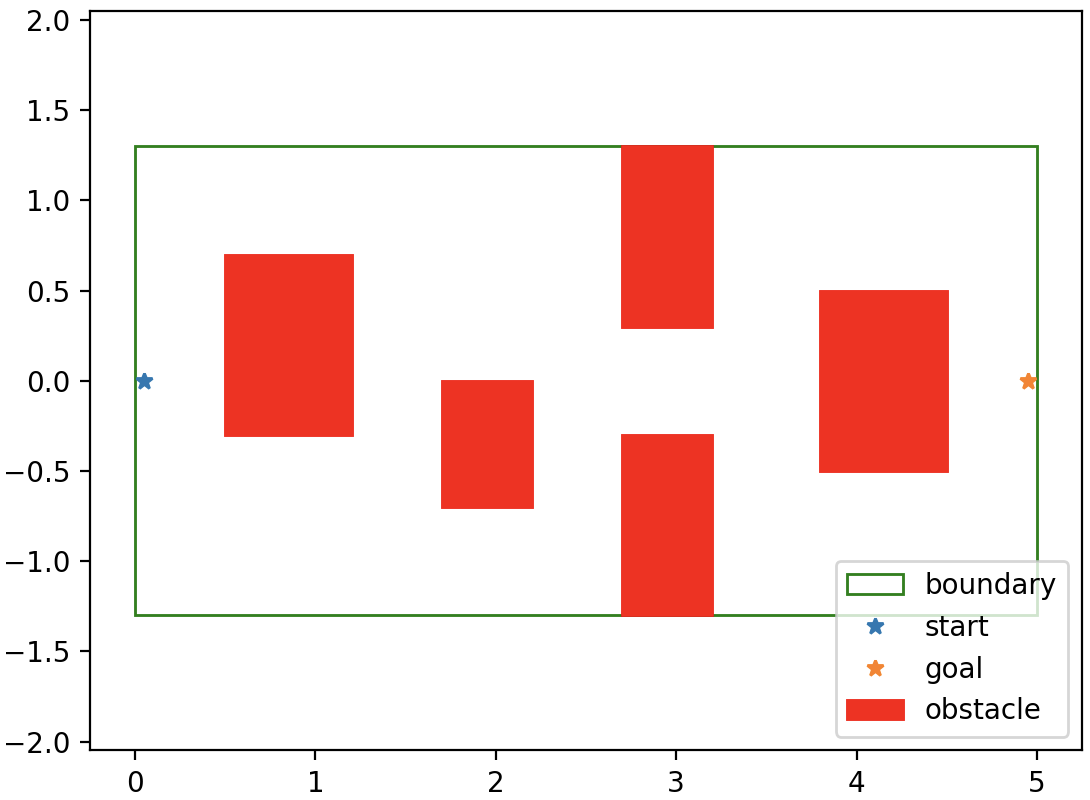
\includegraphics[width=\linewidth]{world.png}
	\caption{Rendering of the vehicle's environment and obstacles.}
\end{figure}

\subsubsection{Motion Planning Problem.} This algorithm constitutes the computational runtime that our neural network seeks to minimize. We structured it as a convex optimization problem in Python using the \texttt{cvxpy} library. The problem is given input Parameters:
\[x,\; x_{goal},\; obs\_lower,\; obs\_size\]

\noindent where the latter two are arrays of \(obs_l\) and \(obs_s\) tuples representing obstacles the vehicle has detected so far. The problem outputs Variables:
\[x_{sol},\; u_{sol},\; b\_l_{sol},\; b\_u_{sol}\]

\noindent which are the optimal state, input, and binary variables for obstacle avoidance that the algorithm solves for. The vehicle's dynamics are modeled by the state matrix \( A \) and input matrix \( B \):
\begin{align*}
    & A = \begin{bmatrix}
        1 & 0 & dt & 0 \\
        0 & 1 & 0 & dt \\
        0 & 0 & 1 & 0  \\
        0 & 0 & 0 & 1
    \end{bmatrix}, \quad
    B = dt \begin{bmatrix}
        0.5 \cdot dt & 0 \\
        0 & 0.5 \cdot dt \\
        1 & 0 \\
        0 & 1
    \end{bmatrix} \\
    & \text{where} \quad x[t+\Delta] = Ax[t] + Bu[t].
\end{align*}

Obstacle avoidance constraints are implemented using the Big-M method. For each obstacle, \(b\_l_{sol}\) and \(b\_u_{sol}\) are introduced, with the matrix \(M\) given by:
\[M = \begin{bmatrix}
2 \cdot max(a_x) & 0 \\
0 & 2 \cdot max(a_y)
\end{bmatrix}\]

\noindent For each obstacle \(i\), binary constraints are given by:
\begin{align*}
    & x[t+\Delta] \leq obs\_lower^{(i)} + M \times b\_l_{sol}^{(i)}[t], \\
    & x[t+\Delta] \geq obs\_upper^{(i)} - M \times b\_u_{sol}^{(i)}[t], \\
    & b\_l_{sol}^{(i)}[0, k] + b\_l_{sol}^{(i)}[1, k] + b\_u_{sol}^{(i)}[0, k] + b\_u_{sol}^{(i)}[1, k] < 4
\end{align*}

\noindent where \(obs\_upper\) is an array of tuples representing the upper right-hand corners of obstacles, formed by the element-wise addition of tuples in \(obs\_lower\) and \(obs\_size\). The last constraint ensures that the vehicle's position is not bounded by all four walls of an obstacle.

Cost constraints are modeled by the state matrix \(Q\), input matrix \(R\), and horizon \(N\) (the number of timesteps \(\Delta\) to calculate starting from current time \(t\):
\[Q = 100 \cdot I_{(4\times4)}, \quad R = 50 \cdot I_{(2\times2)}, \quad N = 25\]

\noindent where the cost function \(C\) is a weighted sum of the deviation from the goal state \(x_{goal}\) and each input \(u[t]\):
\[\sum_{k=0}^{N-1} \left( \| Q (x[t] - x_{goal}) \| + \| R \cdot u[t] \| \right) + p \| x[N] - x_{goal} \|\]

\noindent where \(p\) is a large penalty on the terminal state \(x[N]\) to encourage approaching \(x_{goal}\).
The problem is formulated as minimizing \(C\) subject to the above constraints for (\(t = 0,\; \Delta,\; \ldots,\; \Delta(N-1)\)). This definition allows for an efficient computation of the optimal trajectory, avoiding obstacles while minimizing the cost function.

\section{III. PROPOSED METHOD}

\quad However, the motion planning problem faced computational challenges. While our solutions were effective in simulations, the real-time applications proved impractical. The average computation time for solving the full problem naively was 0.2 seconds, but this could escalate to as much as 2.3 seconds in scenarios involving complex obstacles (Table 1). This delay was critical; by the time the solution was computed, the car had already moved beyond the planned trajectory, often resulting in crashes. This highlighted the need for a more efficient solution suitable for real-world applications.

To address these challenges, we shifted our focus to leveraging neural networks. Our strategy involved training a neural network to predict the binary variables essential for solving the full problem. Traditionally, these variables \(b\_l_{sol}, b\_u_{sol}\) were obtained by solving the complete \texttt{cvxpy} problem. However, in our novel approach, we introduced these variables as parameters into a relaxed \texttt{cvxpy} problem. This method, which we refer to as the 'Model' method, was hypothesized to be significantly faster than the 'Naive' full problem method, thus reducing computational delays.

Our model, developed using PyTorch, was designed to handle 24 input dimensions. These included four values representing the vehicle's state, \(x\), and 20 values from the vehicle's detected obstacles (comprising ten values each from five \(obs_l\) and five \(obs_s\) tuples). The output of the model consisted of 500 dimensions, corresponding to the binary variables in \(b\_l_{sol}, b\_u_{sol}\), calculated as five obstacles times a horizon of N, resulting in 25 values for both x and y coordinates. 

\textit{Side note: A notable aspect of our model is its ability to handle scenarios where fewer than five obstacles are detected. In such cases, we appended dummy obstacles with zero width at the origin to maintain consistent input dimensions.}

The model is a binary classification network with eight linear hidden layers, each comprising 512 neurons. After the input layer, we applied \texttt{torch.nn. BatchNorm1D} normalization. Our initial experiments included \texttt{torch.nn.Dropout(0.1)} after each hidden layer, but this was later removed due to a decline in model performance. We experimented with both relu and leaky relu activation functions, ultimately selecting leaky relu for its superior performance. 

The inclusion of each feature in our model was justified through experimental validation. The exact numbers of layers and neurons were determined to optimize the balance between computational efficiency and the model's ability to accurately predict binary variables.

The model was trained over 256 epochs with a batch size of 2048, using a dataset comprising over \(1.3 \times 10^5\) values. The initial learning rate was set at 0.001. We utilized \texttt{TensorDataset} from \texttt{torch.utils.data} for organizing our data and labels and divided our dataset into an 80\% training and 20\% validation split using \texttt{random\_split}. The \texttt{DataLoader} was employed for handling both training and validation datasets.

In terms of optimizers, we compared the performance of \texttt{optim.Adam} and \texttt{optim.SGD}, eventually choosing Adam due to its superior results. Our loss function was initially \texttt{nn.BCEWithLogitsLoss} during training, which was switched to \texttt{nn.BCELoss} (with a manual sigmoid) for evaluation. We also incorporated positive weighting in our loss function to give preference to 1s over 0s, which proved beneficial. The learning rate was adjusted by a factor of \(\frac{1}{10}\) upon stagnation using the \texttt{ReduceLROnPlateau} scheduler.

The selection of each parameter, including the number of epochs, batch size, and learning rate, was based on extensive experimentation to achieve the best balance between training efficiency and model accuracy.

\section{IV. EXPERIMENTAL SETUP}

\begin{table}
    \caption{Comparison of metrics; 1000 iterations per method.}
    \centering
    \begin{tabular}{l r r}
        \toprule
        Solve Time Metric & Naive Soln. & Model Soln. \\
        \midrule
        Minimum & 0.01844  & 0.003887 \\
        Median  & 0.08775  & 0.005787 \\
        Maximum & 2.2856   & 0.009929 \\
        Average & 0.1868   & 0.005978 \\
        Standard Deviation & 0.3277 & 0.000948 \\
        \bottomrule
    \end{tabular}
\end{table}

\quad To construct a comprehensive dataset for training our model, we engaged in an extensive data collection process. This involved simulating the full motion planning problem over 1500 iterations, each with a randomly assigned starting state for the vehicle. For every timestep $\Delta$ in the range $0 \leq t < t_{end}$, the vehicle's current state $x$, detected obstacles (characterized by $obs\_lower$ and $obs\_size$), and the target state $x_{goal}$ were input into the simulation. The outputs from the simulation, $x_{sol}$ and $u_{sol}$, were then used to update the vehicle's state for the next timestep, following the kinematic equations:
\begin{align*}
    p_{x, y}[1] &= p_{x, y}[0] + v_{x, y}[0] \Delta + \frac{1}{2} (a_{x, y}[0] \cdot \Delta^2) \\
    v_{x, y}[1] &= v_{x, y}[0] + a_{x, y}[0] \Delta
\end{align*}
Additionally, the binary variables $b\_l_{sol}$ and $b\_u_{sol}$ were recorded in the dataset, paired with corresponding values of $x$ and $obs\_lower,\; obs\_size$ as keys.

The dataset, structured as a dictionary of key-value pairs, required minimal preprocessing. The only steps taken were batch normalization and the division of the dataset into training and validation sets, as detailed in Section III above. This streamlined approach ensured that the data was ready for model training without the need for extensive cleaning or modification.

In assessing the performance of our model, we employed a rigorous evaluation methodology. During the training loop, the model was saved at the end of each epoch if its validation loss was lower than that of all previous epochs. Our target was to achieve a loss of 2.5\% or lower, and our best-performing model, as described in Section III, attained a loss of just 2.2\%. 

For benchmarking purposes, we compared our model against the full motion planning problem, treated as our Naive algorithm. The primary benchmark was to surpass the Naive baseline in terms of solve time at each timestep by at least a factor of 10. The average solve time for the Naive solution (across 1000 iterations of the problem) was about 0.2 seconds, as described in Table 1 and visualized in Figure 2.

The implementation of our model was carried out on a physical vehicle using the BARC platform. These \(\frac{1}{10}\) scale model electric cars are equipped with advanced sensors, including LiDar and high-resolution cameras. They are capable of streaming data to an external computing unit for real-time offboard computation. The vehicle operates using the Robotic Operating System, facilitating efficient data handling and model integration. This setup provided a realistic and robust platform for testing and refining our autonomous car's obstacle avoidance and racing capabilities.

\textit{View the source code for this project and demo videos of the BARC at} \texttt{\href{https://github.com/shn66/L4MIMPC_urap}{github.com/shn66/L4MIMPC\_urap}}.

\section{V. RESULTS \& ANALYSIS}

\begin{figure}
	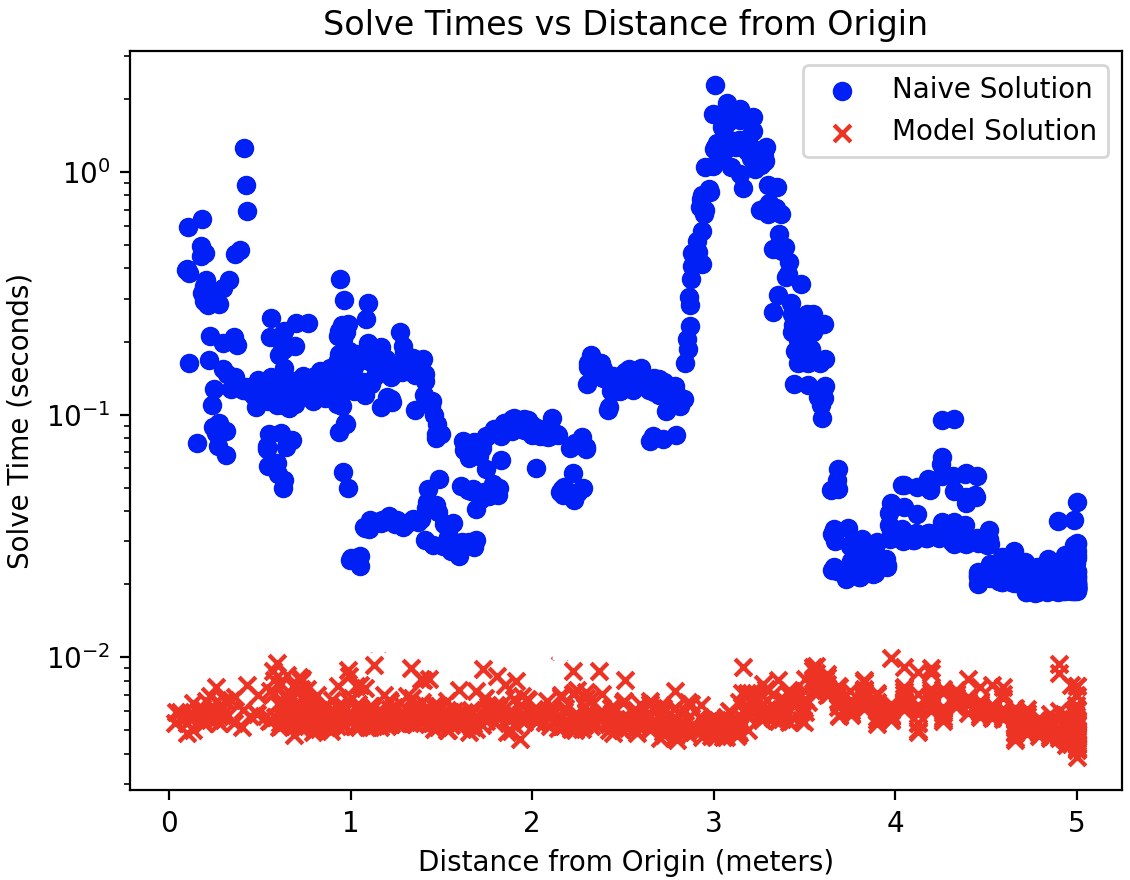
\includegraphics[width=\linewidth]{graph.png}
	\caption{Solve times vs distance from origin for both methods.}
\end{figure}

\quad Performance was further measured by inputting data from the dataset into the model and comparing the number of element-wise discrepancies between the model’s output and the expected binary variables. On average, across all points in the dataset, our model exhibited 1.2 discrepancies out of 250 variables for $bl\_sol$, and 3.6 out of 250 for $bu\_sol$, resulting in a total of 4.8 discrepancies out of 500 for both variables combined. This translates to an impressive accuracy rate of 99.04\%, which proved accurate enough for the model to solve the problem independently with a similar success rate.

Additionally, our Model solution performed significantly better than the benchmark in terms of solve time, averaging 0.006 seconds as shown in Table 1 and Figure 2. Compared to the Naive solution's average of 0.2 seconds, our Model solution reduces solve time by a factor of more than 30, significantly outperforming our baseline and our expectations of a tenfold reduction.

To visualize the Model solution’s improvement over the full problem, we may analyze individual sections of our graphs. A general trend of the Naive solution is that solve times are significantly greater when the vehicle must navigate through tight corridors or around large obstacles, forcing the planned trajectory to calculate a curve instead of simply going straight.

For instance, when the distance from the origin in Figure 2, and by approximation, the distance along the x-axis in Figure 1, is between 0 and 1 meters. A large peak occurs around a tight squeeze at 3 meters. On the other hand, the Model solution successfully reduces those solve times by an order of magnitude as shown in Figure 2, stabilizing around 0.05 seconds regardless of obstacle locations or the vehicle's whereabouts.

In a part-by-part analysis, the model's performance was evaluated under different training conditions and environmental setups. Notably, the model demonstrated robust performance when trained on a large dataset comprising random simulated starting states. However, it exhibited even more refined and accurate behavior when trained on a slightly smaller dataset where the starting points closely mirrored those we chose in the physical testing environment. This suggests that the model's learning is significantly enhanced by training on data that closely resembles real-world scenarios. Furthermore, the model's performance was observed to be superior in environments with fewer obstacles and more constrained settings. This indicates that while the model is capable of handling complex scenarios, its efficiency and accuracy are maximized in simpler and predictable environments.

Our analysis and comparison of the model's performance with baseline and state-of-the-art methods reveal several key insights. Firstly, the model's high accuracy rate of 99.04\% in solving the problem independently is a testament to its robustness and reliability. This level of accuracy is not only significantly higher than that of traditional methods, but also positions our model as a competitive alternative in the field of autonomous vehicle navigation. Additionally, the dramatic reduction in solve time by a factor of over 30 compared to the Naive solution underscores the efficiency of our model. Coupled with the model's ability to maintain stable solve times regardless of environmental complexity, as evidenced in our qualitative analysis, it holds great potential for real-world applications in autonomous car racing and obstacle avoidance. A part-by-part analysis further enriches our understanding of the model's adaptability and efficiency, particularly in scenarios that closely resemble real-world conditions.

\section{VI. CONCLUSION}

\quad Our neural network model, adept at processing minimal input data for high-speed autonomous vehicle operations, holds promise for real-world applications in autonomous racing, advanced driver-assistance systems, and beyond. Its efficiency in high-speed, limited visibility environments marks a significant advancement in autonomous vehicle technology.

Despite its strengths, the model's current design is specific to the BARC platform and may not directly translate to other systems. Its performance in varied environmental conditions also requires further exploration, highlighting scalability challenges. The model does not yet address the adaptability to unpredictable environmental changes or real-time learning from new obstacles, which remains a key challenge in autonomous navigation.

This research pushes the boundaries of neural network applications in time-sensitive scenarios, setting a new benchmark for efficiency and accuracy in machine learning for autonomous vehicles. It contributes significantly to the field, demonstrating the potential of neural networks in complex, real-world tasks.

Future work should focus on enhancing the model's adaptability to diverse environments and integrating reinforcement learning for real-time obstacle adaptation. Expanding its application to different autonomous platforms will also be a crucial step in broadening its impact across various sectors.

%%% REFERENCES %%%

% TODO: Proofread the Abstract and all the Sections and revise
% anything that's confusing; ALSO: google scholar like 12 plus 
% references to sprinkle in the paper, the intro in particular

\cite{citation1} % Cite each source like this for them
\cite{citation2} % to appear in the references section

\printbibliography % See {sample.bib} for the list of sources
% Other stuff like the cls file and formatting should be good
% The math-heavy stuff in Section II we can give to Sid later
\end{document}